%%%%%%%%%%%%%%%%%%%%%%%%%%%%%%%%%%%%%%%%%%%%%%%%%%%%%%%%%%%%%%%%%%%%%%%%%%%%%%%%
% experiment.tex: Chapter describing the experiment
%%%%%%%%%%%%%%%%%%%%%%%%%%%%%%%%%%%%%%%%%%%%%%%%%%%%%%%%%%%%%%%%%%%%%%%%%%%%%%%%
\chapter{HPS}
\label{chapter:hps:experiment}
%%%%%%%%%%%%%%%%%%%%%%%%%%%%%%%%%%%%%%%%%%%%%%%%%%%%%%%%%%%%%%%%%%%%%%%%%%%%%%%%
\ac{hps} is currently installed behind the CLAS-12 experiment in the Hall B
alcove at \ac{jlab} and utilizes the \ac{cebaf} to provide its beam
\cite{mrsolt-thesis-2020,skmccarty-thesis-2020}.
Hall B primarily hosts the CLAS-12 experiment \todo[citation]{Add citation for CLAS-12}
in the bulk of its hall; nevertheless, behind the CLAS-12 experiment \ac{hps} is situated
within an alcove such that it can collect data whenever CLAS-12 is not operational (for example,
when its components are being upgraded or fixed).

\ac{cebaf} \cite{cebaf-12GeV-2012,cebaf-opportunities-2012,cebaf-2013} is able to
provide a near-continuous electron beam ranging in energy up to $12$ GeV in steps
of $\approx 1.15$ GeV. \ac{cebaf} is built in a oval ``race track'' where the straight
portions consist of linear accelerators and the curve portions steer the beam with
dipole magnets either back into the straight portions or into experimental halls.
Since \ac{cebaf} delivers electrons at such a high rate, \ac{hps} must be able to
handle these high radiation loads. Designed to be a small experiment to fit within
the Hall B alcove, \ac{hps} elected to be built in two halves that straddle the primary
path of the beam where the highest amount of radiation would be. Both of the subsystems
within \ac{hps} are split into these two halves as shown in \cref{fig:hps-full-render}
and other diagrams below.

\begin{figure}
    \centering
    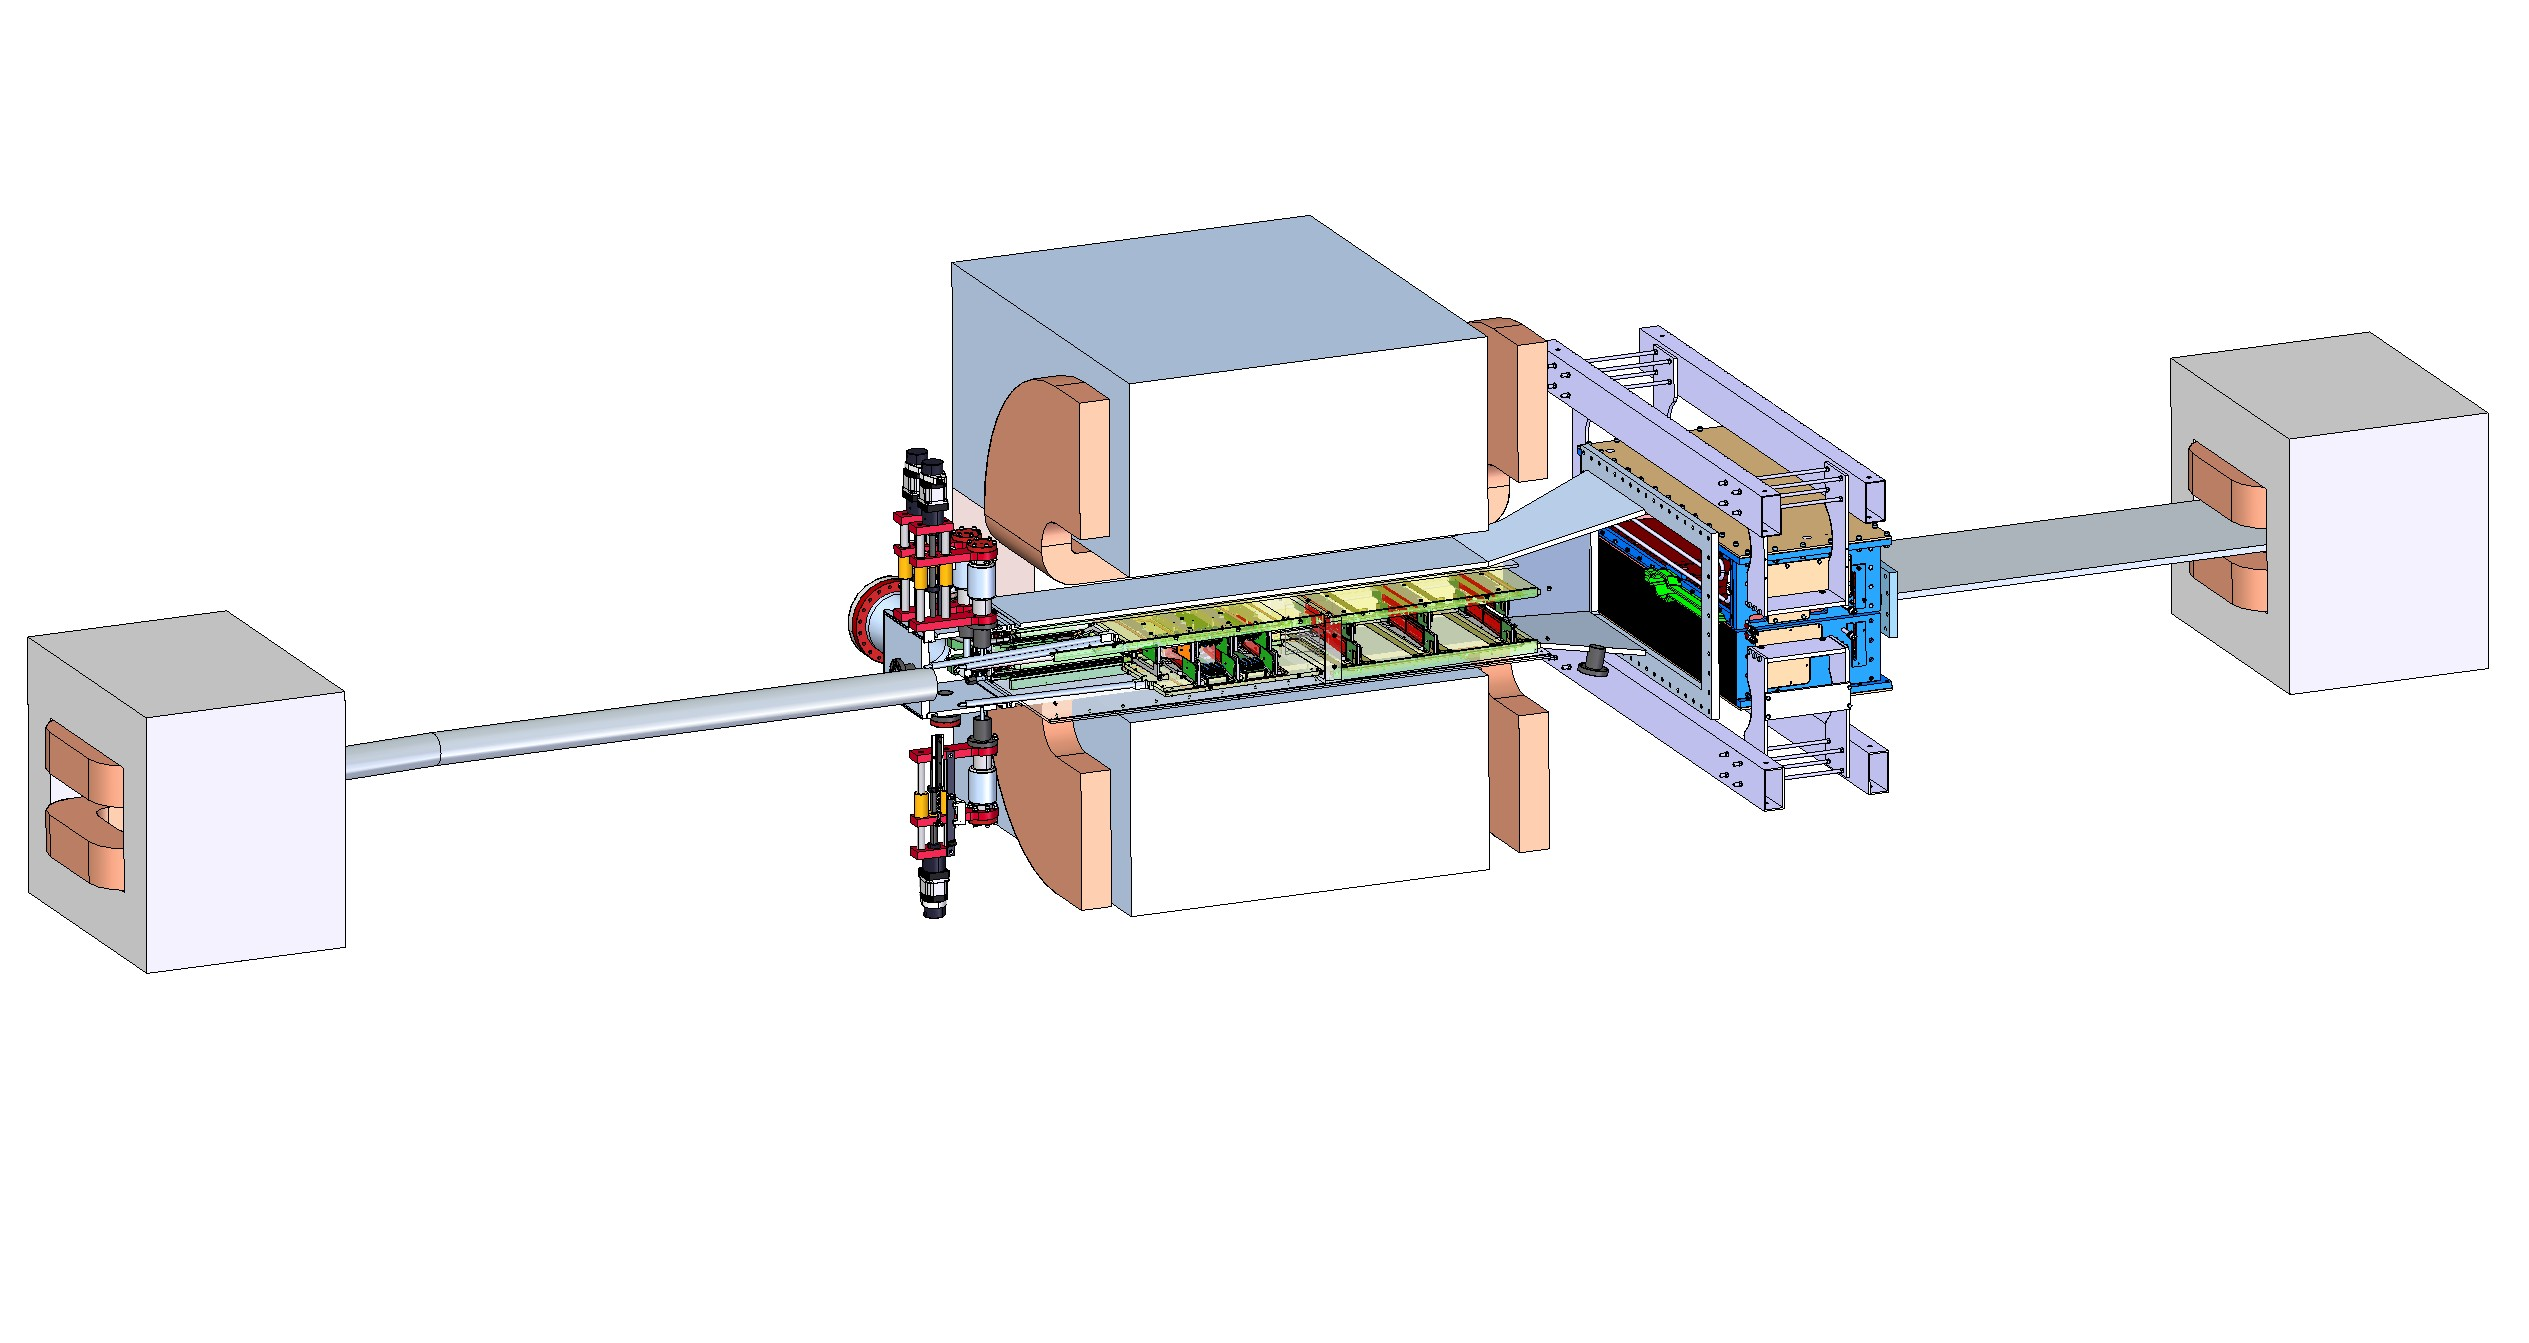
\includegraphics[trim={15cm 10cm 10cm 5cm},clip,width=\textwidth]{figures/hps/experiment/hps_full_render.jpg}
    \caption{
        Full rendering of \ac{hps}.
        Beam would enter the detector from the left and exit to the right if it does not interact.
    }
    \label{fig:hps-full-render}
\end{figure}

\section{Silicon Vertex Tracker}
The \ac{svt}...

\begin{figure}
    \centering
    \includegraphics*[width=\textwidth]{figures/hps/experiment/smkcarty-thesis-fig-10-svt-render.png}
    \caption{
        Figure 10 of \cite{skmccarty-thesis-2020}. Rendering of the \ac{svt} with the vacuum
        enclosure shown in gray, active silicon components in red, and readout electronics in
        green. Similar to \cref{fig:hps-full-render}, the beam would traverse this rendering
        from left to right.
    }
    \label{fig:hps-svt-render}
\end{figure}

\section{Electromagnetic Calorimeter}

\section{Currently-Available Datasets}
